% ============================================================================
% CHƯƠNG 9: LẬP TRÌNH SONG SONG VỚI C#
% ============================================================================
\chapter{Lập trình Song song với C\#}
\label{chap:csharp}

\section{Giới thiệu}

C\# cung cấp nhiều cơ chế lập trình song song mạnh mẽ thông qua .NET Framework:

\begin{itemize}
    \item \textbf{System.Threading}: Thread, ThreadPool, Interlocked
    \item \textbf{Task Parallel Library (TPL)}: Task, Parallel.For, Parallel.ForEach
    \item \textbf{Channels}: Producer-Consumer pattern hiện đại
    \item \textbf{PLINQ}: Parallel LINQ cho collections
    \item \textbf{async/await}: Asynchronous programming model
\end{itemize}

\begin{figure}[H]
\centering
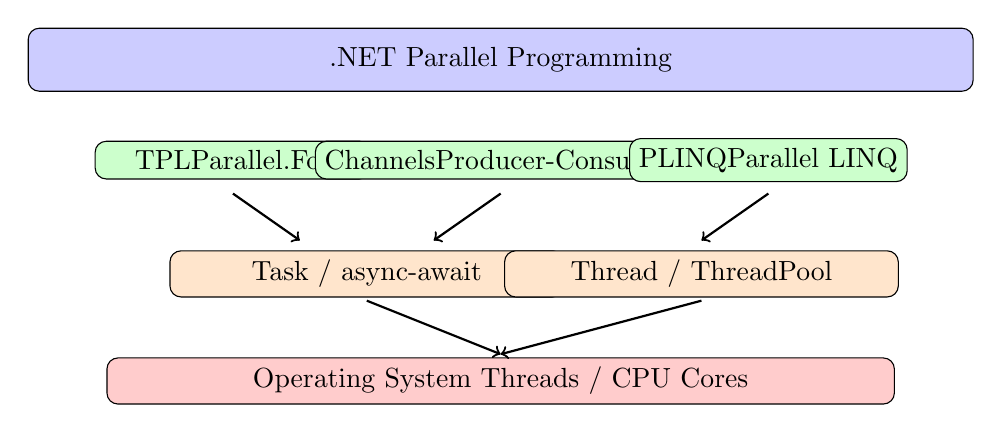
\begin{tikzpicture}[scale=0.85]
    % Hierarchy
    \node[draw, fill=blue!20, rounded corners, minimum width=12cm, minimum height=0.8cm] at (0, 4) {.NET Parallel Programming};
    
    \node[draw, fill=green!20, rounded corners, minimum width=3.5cm] at (-4, 2.5) {TPL\\Parallel.For};
    \node[draw, fill=green!20, rounded corners, minimum width=3.5cm] at (0, 2.5) {Channels\\Producer-Consumer};
    \node[draw, fill=green!20, rounded corners, minimum width=3.5cm] at (4, 2.5) {PLINQ\\Parallel LINQ};
    
    \node[draw, fill=orange!20, rounded corners, minimum width=5cm] at (-2, 0.8) {Task / async-await};
    \node[draw, fill=orange!20, rounded corners, minimum width=5cm] at (3, 0.8) {Thread / ThreadPool};
    
    \node[draw, fill=red!20, rounded corners, minimum width=10cm] at (0, -0.8) {Operating System Threads / CPU Cores};
    
    % Arrows
    \draw[->, thick] (-4, 2) -- (-3, 1.3);
    \draw[->, thick] (0, 2) -- (-1, 1.3);
    \draw[->, thick] (4, 2) -- (3, 1.3);
    \draw[->, thick] (-2, 0.4) -- (0, -0.4);
    \draw[->, thick] (3, 0.4) -- (0, -0.4);
    
\end{tikzpicture}
\caption{Các tầng lập trình song song trong C\#}
\label{fig:csharp_parallel_layers}
\end{figure}

\section{Parallel.For}

\subsection{Cú pháp cơ bản}

\code{Parallel.For} thực thi vòng lặp song song, phân chia iterations cho nhiều threads:

\begin{lstlisting}[style=csharpstyle, caption={Parallel.For cơ bản}, label={lst:parallel_for_basic}]
using System;
using System.Threading.Tasks;

class Program {
    static void Main() {
        // Sequential
        for (int i = 0; i < 10; i++) {
            Console.WriteLine($"Sequential: {i}");
        }
        
        // Parallel - thu tu khong dam bao
        Parallel.For(0, 10, i => {
            Console.WriteLine($"Parallel: {i} on thread {Thread.CurrentThread.ManagedThreadId}");
        });
    }
}
\end{lstlisting}

\subsection{Ví dụ: Tính Factorial}

\begin{lstlisting}[style=csharpstyle, caption={Tính Factorial với Parallel.For}, label={lst:factorial_parallel}]
public class FactorialParallel {
    public static void Run() {
        int n = 10;
        
        // Parallel.For de tinh n! cho cac so tu 0 den n-1
        Parallel.For(0, n, i => {
            long factorial = ComputeFactorial(i);
            Console.WriteLine($"{i}! = {factorial}");
        });
        
        Console.WriteLine("Note: Results may appear in different order");
    }
    
    public static long ComputeFactorial(int num) {
        long result = 1;
        for (int j = 1; j <= num; j++) {
            result *= j;
        }
        return result;
    }
}
\end{lstlisting}

\subsection{Parallel Reduction với Local State}

\begin{lstlisting}[style=csharpstyle, caption={Vector Sum với Local State}, label={lst:vector_sum_parallel}]
public class VectorSumParallel {
    public static void Run() {
        int vectorSize = 1000000;
        int[] vector = Enumerable.Range(1, vectorSize).ToArray();
        
        // Method 1: Interlocked (thread-safe nhung cham)
        long sum1 = 0;
        Parallel.For(0, vectorSize, i => {
            Interlocked.Add(ref sum1, vector[i]);
        });
        
        // Method 2: Local State (hieu qua hon)
        long sum2 = 0;
        object lockObj = new object();
        
        Parallel.For(0, vectorSize,
            // Initialize local state cho moi thread
            () => 0L,
            // Body: tich luy vao local sum
            (i, loopState, localSum) => {
                return localSum + vector[i];
            },
            // Final: combine local sums
            (localSum) => {
                lock (lockObj) {
                    sum2 += localSum;
                }
            }
        );
        
        // Method 3: Partitioning (tot nhat)
        int numPartitions = Environment.ProcessorCount;
        int partitionSize = vectorSize / numPartitions;
        long[] partialSums = new long[numPartitions];
        
        Parallel.For(0, numPartitions, p => {
            int start = p * partitionSize;
            int end = (p == numPartitions - 1) ? vectorSize : start + partitionSize;
            
            long localSum = 0;
            for (int i = start; i < end; i++) {
                localSum += vector[i];
            }
            partialSums[p] = localSum;
        });
        
        long sum3 = partialSums.Sum();
    }
}
\end{lstlisting}

\begin{figure}[H]
\centering
\begin{tikzpicture}[scale=0.8]
    % Partitioning visualization
    \node[font=\bfseries] at (6, 6) {Parallel Reduction với Partitioning};
    
    % Original array
    \draw[fill=blue!10] (0, 4.5) rectangle (12, 5.2);
    \node at (6, 4.85) {Vector [1, 2, 3, ..., N]};
    
    % Partitions
    \foreach \i/\c in {0/red, 1/green, 2/blue, 3/orange} {
        \draw[fill=\c!30] ({\i*3}, 3) rectangle ({(\i+1)*3}, 3.7);
        \node[font=\tiny] at ({\i*3+1.5}, 3.35) {Partition \i};
    }
    
    % Threads
    \foreach \i in {0,1,2,3} {
        \draw[->, thick] ({\i*3+1.5}, 2.9) -- ({\i*3+1.5}, 2.3);
        \node[draw, circle, fill=yellow!50, font=\tiny] at ({\i*3+1.5}, 2) {T\i};
    }
    
    % Local sums
    \foreach \i/\v in {0/S0, 1/S1, 2/S2, 3/S3} {
        \draw[fill=purple!20] ({\i*3+0.7}, 0.8) rectangle ({(\i+1)*3-0.7}, 1.4);
        \node[font=\small] at ({\i*3+1.5}, 1.1) {\v};
    }
    
    % Final reduction
    \draw[->, thick] (1.5, 0.7) -- (5.5, 0);
    \draw[->, thick] (4.5, 0.7) -- (5.5, 0);
    \draw[->, thick] (7.5, 0.7) -- (6.5, 0);
    \draw[->, thick] (10.5, 0.7) -- (6.5, 0);
    
    \node[draw, fill=green!40, minimum width=2cm, font=\bfseries] at (6, -0.5) {Total Sum};
    
\end{tikzpicture}
\caption{Parallel Reduction với Partitioning}
\label{fig:csharp_partitioning}
\end{figure}

\section{Channel (Producer-Consumer Pattern)}

\subsection{Giới thiệu Channels}

Channels trong C\# cung cấp cơ chế giao tiếp an toàn giữa producers và consumers:

\begin{lstlisting}[style=csharpstyle, caption={Channel Producer-Consumer cơ bản}, label={lst:channel_basic}]
using System.Threading.Channels;

// Tao unbounded channel
var channel = Channel.CreateUnbounded<int>();

// Producer
var producer = Task.Run(async () => {
    for (int i = 0; i < 10; i++) {
        await channel.Writer.WriteAsync(i);
        Console.WriteLine($"Produced: {i}");
    }
    channel.Writer.Complete();
});

// Consumer
await foreach (var item in channel.Reader.ReadAllAsync()) {
    Console.WriteLine($"Consumed: {item}");
}
\end{lstlisting}

\subsection{Ví dụ: Tính Factorial với Channel}

\begin{lstlisting}[style=csharpstyle, caption={Factorial với Channel Pattern}, label={lst:factorial_channel}]
public class FactorialChannel {
    public static async Task RunAsync() {
        int n = 10;
        
        // Channel chua (number, factorial) pairs
        var channel = Channel.CreateUnbounded<(int number, long factorial)>();
        var writer = channel.Writer;
        var reader = channel.Reader;
        
        // Producer: Tinh factorials va gui qua channel
        var producerTask = Task.Run(async () => {
            Console.WriteLine("[Producer] Starting...");
            
            for (int i = 0; i < n; i++) {
                long factorial = ComputeFactorial(i);
                await writer.WriteAsync((i, factorial));
                Console.WriteLine($"[Producer] Sent: {i}! = {factorial}");
            }
            
            writer.Complete();  // Signal ket thuc
            Console.WriteLine("[Producer] Completed.");
        });
        
        // Consumer: Doc results tu channel
        Console.WriteLine("[Consumer] Starting...");
        await foreach (var item in reader.ReadAllAsync()) {
            Console.WriteLine($"[Consumer] Received: {item.number}! = {item.factorial}");
        }
        Console.WriteLine("[Consumer] Finished.");
        
        await producerTask;
    }
}
\end{lstlisting}

\begin{figure}[H]
\centering
\begin{tikzpicture}[scale=0.85]
    % Producer
    \node[draw, fill=blue!30, rounded corners, minimum width=2.5cm, minimum height=1.5cm] (P) at (0, 0) {Producer};
    
    % Channel (queue)
    \node[draw, fill=orange!30, minimum width=4cm, minimum height=1cm] (C) at (5, 0) {};
    \node[above] at (5, 0.6) {Channel (Queue)};
    \foreach \i in {0,1,2} {
        \draw[fill=yellow!50] ({3.5+\i*0.8}, -0.3) rectangle ++({0.7}, 0.6);
    }
    
    % Consumer
    \node[draw, fill=green!30, rounded corners, minimum width=2.5cm, minimum height=1.5cm] (Con) at (10, 0) {Consumer};
    
    % Arrows
    \draw[->, very thick, blue] (1.5, 0) -- (3, 0) node[midway, above] {WriteAsync};
    \draw[->, very thick, green!50!black] (7, 0) -- (8.5, 0) node[midway, above] {ReadAllAsync};
    
    % Labels
    \node[below, font=\small] at (0, -1) {Tạo data};
    \node[below, font=\small] at (5, -1) {Buffer};
    \node[below, font=\small] at (10, -1) {Xử lý data};
    
\end{tikzpicture}
\caption{Channel Producer-Consumer Pattern}
\label{fig:channel_pattern}
\end{figure}

\section{PLINQ (Parallel LINQ)}

PLINQ cho phép chạy các LINQ queries song song một cách đơn giản:

\begin{lstlisting}[style=csharpstyle, caption={PLINQ Examples}, label={lst:plinq_examples}]
using System.Linq;

int[] numbers = Enumerable.Range(1, 1000000).ToArray();

// PLINQ Sum
long plinqSum = numbers.AsParallel().Sum(x => (long)x);

// PLINQ with Where and Select
var results = numbers.AsParallel()
    .Where(x => x % 2 == 0)
    .Select(x => x * x)
    .ToArray();

// PLINQ with degree of parallelism
var results2 = numbers.AsParallel()
    .WithDegreeOfParallelism(4)
    .Where(x => x > 500000)
    .Sum();

// PLINQ ForAll (action on each element)
numbers.AsParallel().ForAll(x => {
    if (x % 100000 == 0) {
        Console.WriteLine($"Processing: {x}");
    }
});
\end{lstlisting}

\section{So sánh các phương pháp}

\begin{table}[H]
\centering
\caption{So sánh các phương pháp song song trong C\#}
\label{tab:csharp_comparison}
\begin{tabular}{@{}lccc@{}}
\toprule
\textbf{Phương pháp} & \textbf{Use case} & \textbf{Ưu điểm} & \textbf{Nhược điểm} \\
\midrule
Parallel.For & Data parallelism & Đơn giản, hiệu quả & Không async \\
Channel & Producer-Consumer & Decoupled, async & Overhead nhỏ \\
PLINQ & Collection queries & Cú pháp LINQ & Không kiểm soát \\
Task & Fine-grained control & Linh hoạt & Phức tạp hơn \\
\bottomrule
\end{tabular}
\end{table}

\begin{table}[H]
\centering
\caption{Benchmark: Vector Sum (N = 1,000,000)}
\label{tab:csharp_benchmark}
\begin{tabular}{@{}lcc@{}}
\toprule
\textbf{Method} & \textbf{Time (ms)} & \textbf{Speedup} \\
\midrule
Sequential & 8.2 & 1.0x \\
Parallel.For (Interlocked) & 45.3 & 0.18x (slower!) \\
Parallel.For (Local State) & 3.1 & 2.6x \\
Parallel.For (Partitioning) & 2.4 & 3.4x \\
PLINQ & 2.8 & 2.9x \\
\bottomrule
\end{tabular}
\end{table}

\begin{figure}[H]
\centering
\begin{tikzpicture}
\begin{axis}[
    width=12cm,
    height=7cm,
    xlabel={Phương pháp},
    ylabel={Thời gian (ms)},
    title={So sánh thời gian Vector Sum các phương pháp},
    ybar,
    bar width=25pt,
    symbolic x coords={Sequential, Interlocked, LocalState, Partition, PLINQ},
    xtick=data,
    xticklabel style={rotate=30, anchor=east},
    nodes near coords,
    ymin=0,
    ymax=50,
]
\addplot[fill=blue!60] coordinates {
    (Sequential, 8.2)
    (Interlocked, 45.3)
    (LocalState, 3.1)
    (Partition, 2.4)
    (PLINQ, 2.8)
};
\end{axis}
\end{tikzpicture}
\caption{Benchmark các phương pháp Parallel trong C\#}
\label{fig:csharp_benchmark}
\end{figure}

\section{Best Practices}

\subsection{Khi nào sử dụng mỗi phương pháp}

\begin{enumerate}
    \item \textbf{Parallel.For với Partitioning}: Reduction operations, large arrays
    \item \textbf{Channel}: Streaming data, pipeline processing
    \item \textbf{PLINQ}: Complex queries trên collections
    \item \textbf{async/await}: I/O-bound operations
\end{enumerate}

\subsection{Tránh các lỗi phổ biến}

\begin{lstlisting}[style=csharpstyle, caption={Anti-patterns và Solutions}, label={lst:antipatterns}]
// Anti-pattern 1: Race condition
int sum = 0;
Parallel.For(0, n, i => {
    sum += array[i];  // WRONG: race condition
});

// Solution: Use Interlocked or Local State
Parallel.For(0, n, 
    () => 0,
    (i, state, local) => local + array[i],
    (local) => Interlocked.Add(ref sum, local)
);

// Anti-pattern 2: Parallel for small data
Parallel.For(0, 10, i => {  // WRONG: overhead > benefit
    DoSmallWork(i);
});

// Solution: Only parallelize for large data
if (n > 10000) {
    Parallel.For(0, n, i => DoWork(i));
} else {
    for (int i = 0; i < n; i++) DoWork(i);
}

// Anti-pattern 3: Shared mutable state
List<int> results = new List<int>();
Parallel.For(0, n, i => {
    results.Add(Compute(i));  // WRONG: List not thread-safe
});

// Solution: Use ConcurrentBag or aggregate
ConcurrentBag<int> safeResults = new ConcurrentBag<int>();
Parallel.For(0, n, i => {
    safeResults.Add(Compute(i));
});
\end{lstlisting}

\section{So sánh C\# Parallel với CUDA}

\begin{table}[H]
\centering
\caption{So sánh C\# Parallel và CUDA}
\label{tab:csharp_vs_cuda}
\begin{tabular}{@{}lcc@{}}
\toprule
\textbf{Tiêu chí} & \textbf{C\# Parallel} & \textbf{CUDA} \\
\midrule
Platform & CPU (multi-core) & GPU (many-core) \\
Threads & 4-64 & 1000s \\
Memory model & Shared memory & Hierarchical \\
Ease of use & Dễ & Khó hơn \\
Best for & General parallel & Data-intensive \\
Speedup (typical) & 2-8x & 10-100x \\
\bottomrule
\end{tabular}
\end{table}

\section{Kết luận chương}

Chương này đã trình bày các công cụ lập trình song song trong C\#:

\begin{enumerate}
    \item \textbf{Parallel.For}: Data parallelism với local state và partitioning
    \item \textbf{Channel}: Producer-Consumer pattern hiện đại và async
    \item \textbf{PLINQ}: Song song hóa LINQ queries đơn giản
\end{enumerate}

\textbf{Key takeaways:}
\begin{itemize}
    \item Tránh shared mutable state - sử dụng local state và combine
    \item Interlocked gây contention - sử dụng partitioning thay thế
    \item PLINQ tiện nhưng ít kiểm soát hơn Parallel.For
    \item Channel phù hợp cho pipeline và streaming scenarios
    \item Chỉ parallelize khi data đủ lớn (overhead > benefit)
\end{itemize}
